% Options for packages loaded elsewhere
\PassOptionsToPackage{unicode}{hyperref}
\PassOptionsToPackage{hyphens}{url}
%
\documentclass[
]{article}
\usepackage{amsmath,amssymb}
\usepackage{lmodern}
\usepackage{ifxetex,ifluatex}
\ifnum 0\ifxetex 1\fi\ifluatex 1\fi=0 % if pdftex
  \usepackage[T1]{fontenc}
  \usepackage[utf8]{inputenc}
  \usepackage{textcomp} % provide euro and other symbols
\else % if luatex or xetex
  \usepackage{unicode-math}
  \defaultfontfeatures{Scale=MatchLowercase}
  \defaultfontfeatures[\rmfamily]{Ligatures=TeX,Scale=1}
\fi
% Use upquote if available, for straight quotes in verbatim environments
\IfFileExists{upquote.sty}{\usepackage{upquote}}{}
\IfFileExists{microtype.sty}{% use microtype if available
  \usepackage[]{microtype}
  \UseMicrotypeSet[protrusion]{basicmath} % disable protrusion for tt fonts
}{}
\makeatletter
\@ifundefined{KOMAClassName}{% if non-KOMA class
  \IfFileExists{parskip.sty}{%
    \usepackage{parskip}
  }{% else
    \setlength{\parindent}{0pt}
    \setlength{\parskip}{6pt plus 2pt minus 1pt}}
}{% if KOMA class
  \KOMAoptions{parskip=half}}
\makeatother
\usepackage{xcolor}
\IfFileExists{xurl.sty}{\usepackage{xurl}}{} % add URL line breaks if available
\IfFileExists{bookmark.sty}{\usepackage{bookmark}}{\usepackage{hyperref}}
\hypersetup{
  pdftitle={Oncase2b},
  pdfauthor={Pedro},
  hidelinks,
  pdfcreator={LaTeX via pandoc}}
\urlstyle{same} % disable monospaced font for URLs
\usepackage[margin=1in]{geometry}
\usepackage{color}
\usepackage{fancyvrb}
\newcommand{\VerbBar}{|}
\newcommand{\VERB}{\Verb[commandchars=\\\{\}]}
\DefineVerbatimEnvironment{Highlighting}{Verbatim}{commandchars=\\\{\}}
% Add ',fontsize=\small' for more characters per line
\usepackage{framed}
\definecolor{shadecolor}{RGB}{248,248,248}
\newenvironment{Shaded}{\begin{snugshade}}{\end{snugshade}}
\newcommand{\AlertTok}[1]{\textcolor[rgb]{0.94,0.16,0.16}{#1}}
\newcommand{\AnnotationTok}[1]{\textcolor[rgb]{0.56,0.35,0.01}{\textbf{\textit{#1}}}}
\newcommand{\AttributeTok}[1]{\textcolor[rgb]{0.77,0.63,0.00}{#1}}
\newcommand{\BaseNTok}[1]{\textcolor[rgb]{0.00,0.00,0.81}{#1}}
\newcommand{\BuiltInTok}[1]{#1}
\newcommand{\CharTok}[1]{\textcolor[rgb]{0.31,0.60,0.02}{#1}}
\newcommand{\CommentTok}[1]{\textcolor[rgb]{0.56,0.35,0.01}{\textit{#1}}}
\newcommand{\CommentVarTok}[1]{\textcolor[rgb]{0.56,0.35,0.01}{\textbf{\textit{#1}}}}
\newcommand{\ConstantTok}[1]{\textcolor[rgb]{0.00,0.00,0.00}{#1}}
\newcommand{\ControlFlowTok}[1]{\textcolor[rgb]{0.13,0.29,0.53}{\textbf{#1}}}
\newcommand{\DataTypeTok}[1]{\textcolor[rgb]{0.13,0.29,0.53}{#1}}
\newcommand{\DecValTok}[1]{\textcolor[rgb]{0.00,0.00,0.81}{#1}}
\newcommand{\DocumentationTok}[1]{\textcolor[rgb]{0.56,0.35,0.01}{\textbf{\textit{#1}}}}
\newcommand{\ErrorTok}[1]{\textcolor[rgb]{0.64,0.00,0.00}{\textbf{#1}}}
\newcommand{\ExtensionTok}[1]{#1}
\newcommand{\FloatTok}[1]{\textcolor[rgb]{0.00,0.00,0.81}{#1}}
\newcommand{\FunctionTok}[1]{\textcolor[rgb]{0.00,0.00,0.00}{#1}}
\newcommand{\ImportTok}[1]{#1}
\newcommand{\InformationTok}[1]{\textcolor[rgb]{0.56,0.35,0.01}{\textbf{\textit{#1}}}}
\newcommand{\KeywordTok}[1]{\textcolor[rgb]{0.13,0.29,0.53}{\textbf{#1}}}
\newcommand{\NormalTok}[1]{#1}
\newcommand{\OperatorTok}[1]{\textcolor[rgb]{0.81,0.36,0.00}{\textbf{#1}}}
\newcommand{\OtherTok}[1]{\textcolor[rgb]{0.56,0.35,0.01}{#1}}
\newcommand{\PreprocessorTok}[1]{\textcolor[rgb]{0.56,0.35,0.01}{\textit{#1}}}
\newcommand{\RegionMarkerTok}[1]{#1}
\newcommand{\SpecialCharTok}[1]{\textcolor[rgb]{0.00,0.00,0.00}{#1}}
\newcommand{\SpecialStringTok}[1]{\textcolor[rgb]{0.31,0.60,0.02}{#1}}
\newcommand{\StringTok}[1]{\textcolor[rgb]{0.31,0.60,0.02}{#1}}
\newcommand{\VariableTok}[1]{\textcolor[rgb]{0.00,0.00,0.00}{#1}}
\newcommand{\VerbatimStringTok}[1]{\textcolor[rgb]{0.31,0.60,0.02}{#1}}
\newcommand{\WarningTok}[1]{\textcolor[rgb]{0.56,0.35,0.01}{\textbf{\textit{#1}}}}
\usepackage{graphicx}
\makeatletter
\def\maxwidth{\ifdim\Gin@nat@width>\linewidth\linewidth\else\Gin@nat@width\fi}
\def\maxheight{\ifdim\Gin@nat@height>\textheight\textheight\else\Gin@nat@height\fi}
\makeatother
% Scale images if necessary, so that they will not overflow the page
% margins by default, and it is still possible to overwrite the defaults
% using explicit options in \includegraphics[width, height, ...]{}
\setkeys{Gin}{width=\maxwidth,height=\maxheight,keepaspectratio}
% Set default figure placement to htbp
\makeatletter
\def\fps@figure{htbp}
\makeatother
\setlength{\emergencystretch}{3em} % prevent overfull lines
\providecommand{\tightlist}{%
  \setlength{\itemsep}{0pt}\setlength{\parskip}{0pt}}
\setcounter{secnumdepth}{-\maxdimen} % remove section numbering
\ifluatex
  \usepackage{selnolig}  % disable illegal ligatures
\fi

\title{Oncase2b}
\author{Pedro}
\date{25/01/2022}

\begin{document}
\maketitle

\begin{Shaded}
\begin{Highlighting}[]
\FunctionTok{library}\NormalTok{(tidyverse)}
\end{Highlighting}
\end{Shaded}

\begin{verbatim}
## Warning: package 'tidyverse' was built under R version 4.1.2
\end{verbatim}

\begin{verbatim}
## -- Attaching packages --------------------------------------- tidyverse 1.3.1 --
\end{verbatim}

\begin{verbatim}
## v ggplot2 3.3.5     v purrr   0.3.4
## v tibble  3.1.6     v dplyr   1.0.7
## v tidyr   1.1.4     v stringr 1.4.0
## v readr   2.1.1     v forcats 0.5.1
\end{verbatim}

\begin{verbatim}
## Warning: package 'ggplot2' was built under R version 4.1.2
\end{verbatim}

\begin{verbatim}
## Warning: package 'tibble' was built under R version 4.1.2
\end{verbatim}

\begin{verbatim}
## Warning: package 'tidyr' was built under R version 4.1.2
\end{verbatim}

\begin{verbatim}
## Warning: package 'readr' was built under R version 4.1.2
\end{verbatim}

\begin{verbatim}
## Warning: package 'purrr' was built under R version 4.1.2
\end{verbatim}

\begin{verbatim}
## Warning: package 'dplyr' was built under R version 4.1.2
\end{verbatim}

\begin{verbatim}
## Warning: package 'stringr' was built under R version 4.1.2
\end{verbatim}

\begin{verbatim}
## Warning: package 'forcats' was built under R version 4.1.2
\end{verbatim}

\begin{verbatim}
## -- Conflicts ------------------------------------------ tidyverse_conflicts() --
## x dplyr::filter() masks stats::filter()
## x dplyr::lag()    masks stats::lag()
\end{verbatim}

\begin{Shaded}
\begin{Highlighting}[]
\FunctionTok{library}\NormalTok{(forecast)}
\end{Highlighting}
\end{Shaded}

\begin{verbatim}
## Warning: package 'forecast' was built under R version 4.1.2
\end{verbatim}

\begin{verbatim}
## Registered S3 method overwritten by 'quantmod':
##   method            from
##   as.zoo.data.frame zoo
\end{verbatim}

\begin{Shaded}
\begin{Highlighting}[]
\FunctionTok{library}\NormalTok{(ggplot2)}
\FunctionTok{library}\NormalTok{(seasonal)}
\end{Highlighting}
\end{Shaded}

\begin{verbatim}
## Warning: package 'seasonal' was built under R version 4.1.2
\end{verbatim}

\begin{verbatim}
## 
## Attaching package: 'seasonal'
\end{verbatim}

\begin{verbatim}
## The following object is masked from 'package:tibble':
## 
##     view
\end{verbatim}

\begin{Shaded}
\begin{Highlighting}[]
\FunctionTok{library}\NormalTok{(seasonalview)}
\end{Highlighting}
\end{Shaded}

\begin{verbatim}
## Warning: package 'seasonalview' was built under R version 4.1.2
\end{verbatim}

\begin{verbatim}
## 
## Attaching package: 'seasonalview'
\end{verbatim}

\begin{verbatim}
## The following object is masked from 'package:seasonal':
## 
##     view
\end{verbatim}

\begin{verbatim}
## The following object is masked from 'package:tibble':
## 
##     view
\end{verbatim}

\begin{Shaded}
\begin{Highlighting}[]
\FunctionTok{library}\NormalTok{(urca)}
\end{Highlighting}
\end{Shaded}

\begin{verbatim}
## Warning: package 'urca' was built under R version 4.1.2
\end{verbatim}

\begin{Shaded}
\begin{Highlighting}[]
\FunctionTok{library}\NormalTok{(readxl)}
\end{Highlighting}
\end{Shaded}

\begin{verbatim}
## Warning: package 'readxl' was built under R version 4.1.2
\end{verbatim}

\begin{Shaded}
\begin{Highlighting}[]
\NormalTok{serie\_tempo\_2b }\OtherTok{\textless{}{-}} \FunctionTok{read\_excel}\NormalTok{(}\StringTok{"\textasciitilde{}/Job/Oncase desafio/serie\_tempo\_2b.xlsx"}\NormalTok{)}
\CommentTok{\#View(serie\_tempo\_2b)}
\end{Highlighting}
\end{Shaded}

Transformando o data frame numa série temporal

\begin{Shaded}
\begin{Highlighting}[]
\NormalTok{ts\_2b }\OtherTok{=} \FunctionTok{ts}\NormalTok{(serie\_tempo\_2b}\SpecialCharTok{$}\NormalTok{faturamento, }\AttributeTok{start =} \FunctionTok{c}\NormalTok{(}\DecValTok{2020}\NormalTok{,}\DecValTok{1}\NormalTok{), }\AttributeTok{end =} \FunctionTok{c}\NormalTok{(}\DecValTok{2021}\NormalTok{,}\DecValTok{9}\NormalTok{), }\AttributeTok{frequency=}\DecValTok{365}\NormalTok{)}
\end{Highlighting}
\end{Shaded}

Verificando a existência de sazonalidade

\begin{Shaded}
\begin{Highlighting}[]
\FunctionTok{autoplot}\NormalTok{(ts\_2b)}
\end{Highlighting}
\end{Shaded}

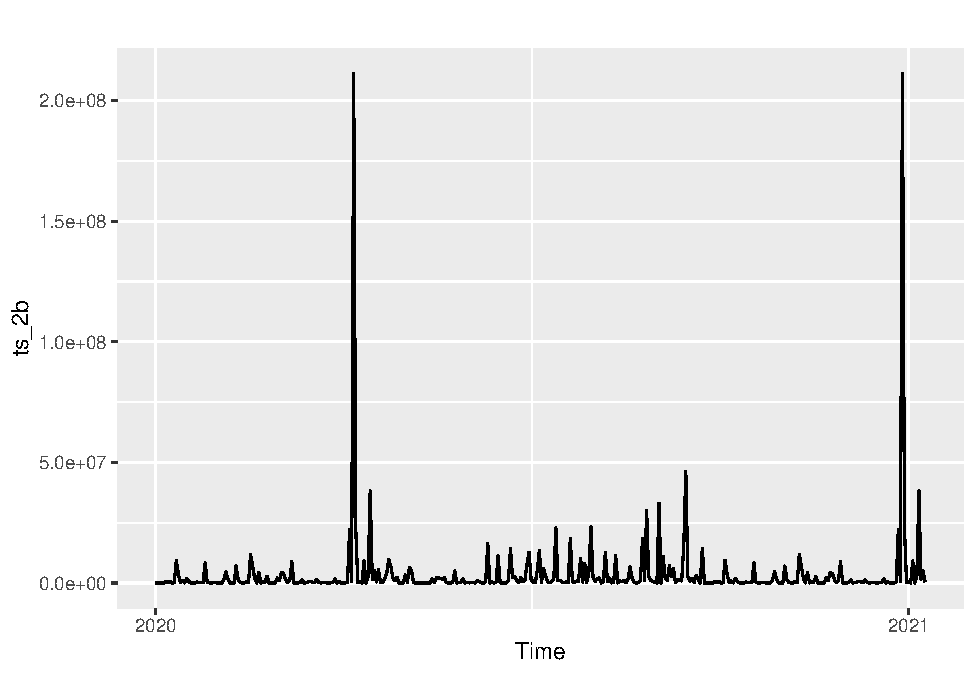
\includegraphics{Oncase2b_files/figure-latex/unnamed-chunk-4-1.pdf}

\begin{Shaded}
\begin{Highlighting}[]
\FunctionTok{hist}\NormalTok{(ts\_2b)}
\end{Highlighting}
\end{Shaded}

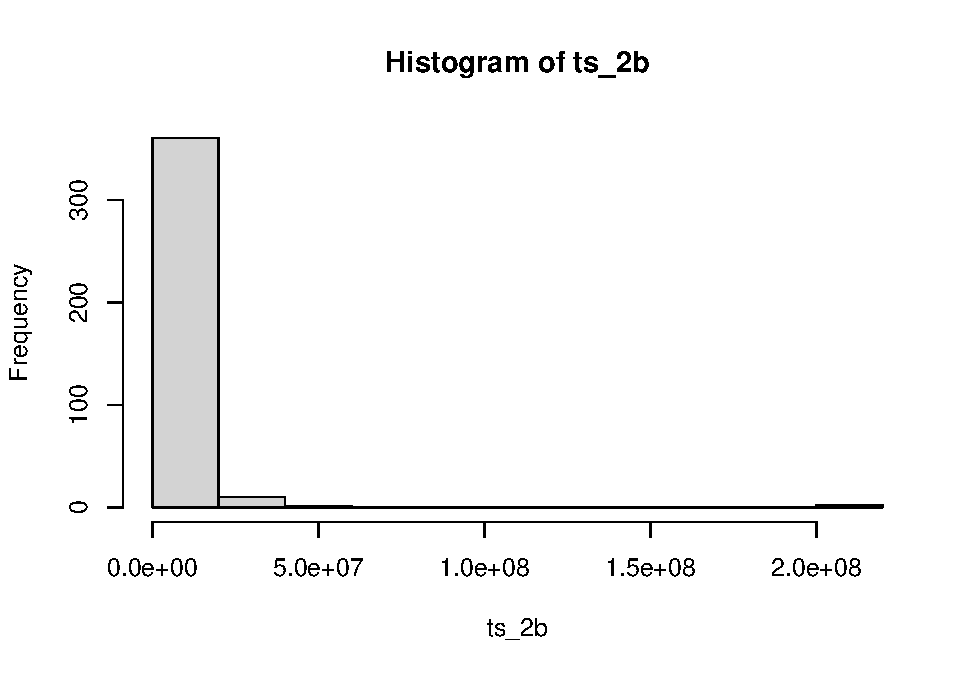
\includegraphics{Oncase2b_files/figure-latex/unnamed-chunk-4-2.pdf}

\begin{Shaded}
\begin{Highlighting}[]
\FunctionTok{boxplot}\NormalTok{(ts\_2b)}
\end{Highlighting}
\end{Shaded}

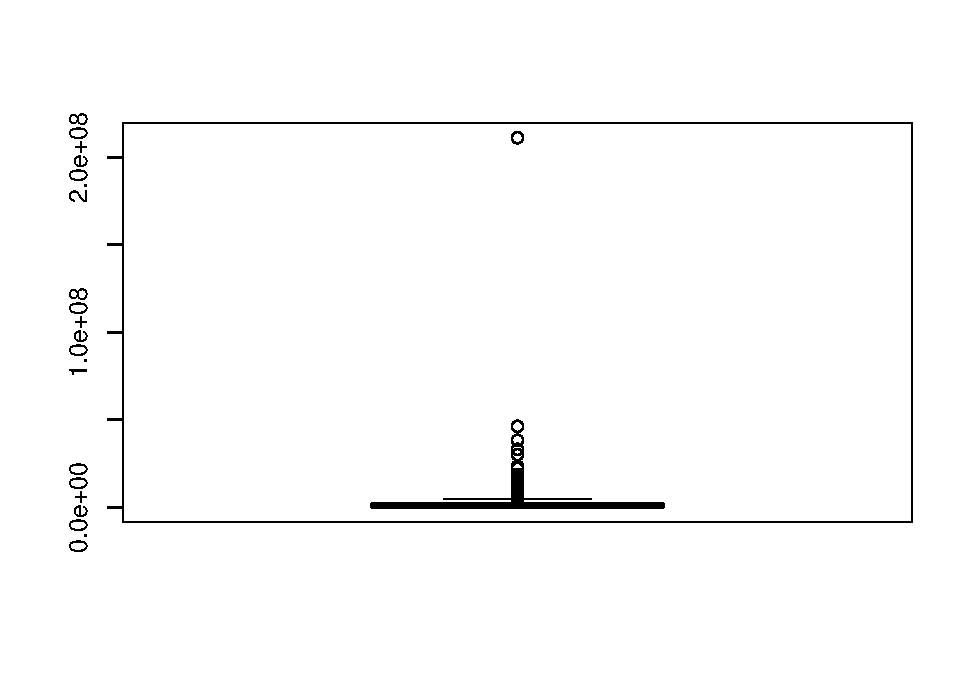
\includegraphics{Oncase2b_files/figure-latex/unnamed-chunk-4-3.pdf}

Segue abaixo uma análise de decomposição da série em estudo.

\begin{Shaded}
\begin{Highlighting}[]
\CommentTok{\#dec =   decompose(ts\_2b)}
\CommentTok{\#autoplot(dec)}
\end{Highlighting}
\end{Shaded}

Percebe-se que não é possível decompor a série pois ela não tem mais de
1 período.

gerou um autoplot da decomposi??o acima observar se existe um padr?o de
sazonalidade e verificar a regularidade

Foram realizadas algumas tentativas de avaliar a existência de
sazonalidad porém não foi possível por não ter mais de um período na
série.

\begin{Shaded}
\begin{Highlighting}[]
\CommentTok{\#ggseasonplot(ts\_2b)}
\CommentTok{\#ggseasonplot(window(ts\_2b, start=c(2021)))}
\end{Highlighting}
\end{Shaded}

\#teste de estacionariedade

\begin{Shaded}
\begin{Highlighting}[]
\NormalTok{est }\OtherTok{=} \FunctionTok{ur.kpss}\NormalTok{(ts\_2b)}
\FunctionTok{print}\NormalTok{(est)}
\end{Highlighting}
\end{Shaded}

\begin{verbatim}
## 
## ####################################### 
## # KPSS Unit Root / Cointegration Test # 
## ####################################### 
## 
## The value of the test statistic is: 0.1174
\end{verbatim}

\begin{Shaded}
\begin{Highlighting}[]
\FunctionTok{ndiffs}\NormalTok{(ts\_2b)}
\end{Highlighting}
\end{Shaded}

\begin{verbatim}
## [1] 0
\end{verbatim}

\begin{Shaded}
\begin{Highlighting}[]
\FunctionTok{tsdisplay}\NormalTok{(ts\_2b)}
\end{Highlighting}
\end{Shaded}

\includegraphics{Oncase2b_files/figure-latex/unnamed-chunk-8-1.pdf}

\begin{Shaded}
\begin{Highlighting}[]
\NormalTok{modelo }\OtherTok{=} \FunctionTok{auto.arima}\NormalTok{(ts\_2b, }\AttributeTok{trace =}\NormalTok{ T,}\AttributeTok{stepwise =}\NormalTok{ F, }\AttributeTok{approximation =}\NormalTok{ F )}
\end{Highlighting}
\end{Shaded}

\begin{verbatim}
## Warning: The chosen seasonal unit root test encountered an error when testing for the first difference.
## From stl(): series is not periodic or has less than two periods
## 0 seasonal differences will be used. Consider using a different unit root test.
\end{verbatim}

\begin{verbatim}
## 
##  ARIMA(0,0,0)             with zero mean     : 13502.73
##  ARIMA(0,0,0)             with non-zero mean : 13486.17
##  ARIMA(0,0,1)             with zero mean     : 13500.31
##  ARIMA(0,0,1)             with non-zero mean : 13486.36
##  ARIMA(0,0,2)             with zero mean     : 13497.74
##  ARIMA(0,0,2)             with non-zero mean : 13486.31
##  ARIMA(0,0,3)             with zero mean     : 13499.64
##  ARIMA(0,0,3)             with non-zero mean : 13488.27
##  ARIMA(0,0,4)             with zero mean     : 13501.68
##  ARIMA(0,0,4)             with non-zero mean : 13490.08
##  ARIMA(0,0,5)             with zero mean     : 13502.75
##  ARIMA(0,0,5)             with non-zero mean : 13491.88
##  ARIMA(1,0,0)             with zero mean     : 13499.36
##  ARIMA(1,0,0)             with non-zero mean : 13486.11
##  ARIMA(1,0,1) with zero mean     : Inf
##  ARIMA(1,0,1)             with non-zero mean : 13487.39
##  ARIMA(1,0,2)             with zero mean     : 13499.59
##  ARIMA(1,0,2)             with non-zero mean : 13488.32
##  ARIMA(1,0,3)             with zero mean     : Inf
##  ARIMA(1,0,3)             with non-zero mean : 13490.24
##  ARIMA(1,0,4)             with zero mean     : Inf
##  ARIMA(1,0,4)             with non-zero mean : 13491.97
##  ARIMA(2,0,0)             with zero mean     : 13497.48
##  ARIMA(2,0,0)             with non-zero mean : 13486.58
##  ARIMA(2,0,1)             with zero mean     : 13499.49
##  ARIMA(2,0,1)             with non-zero mean : 13488.52
##  ARIMA(2,0,2) with zero mean     : Inf
##  ARIMA(2,0,2) with non-zero mean : Inf
##  ARIMA(2,0,3) with zero mean     : Inf
##  ARIMA(2,0,3)             with non-zero mean : Inf
##  ARIMA(3,0,0)             with zero mean     : 13499.49
##  ARIMA(3,0,0)             with non-zero mean : 13488.38
##  ARIMA(3,0,1)             with zero mean     : Inf
##  ARIMA(3,0,1)             with non-zero mean : 13490.3
##  ARIMA(3,0,2)             with zero mean     : Inf
##  ARIMA(3,0,2)             with non-zero mean : Inf
##  ARIMA(4,0,0)             with zero mean     : 13501.54
##  ARIMA(4,0,0)             with non-zero mean : 13490.03
##  ARIMA(4,0,1)             with zero mean     : Inf
##  ARIMA(4,0,1)             with non-zero mean : 13491.96
##  ARIMA(5,0,0)             with zero mean     : 13502.4
##  ARIMA(5,0,0)             with non-zero mean : 13491.91
## 
## 
## 
##  Best model: ARIMA(1,0,0)             with non-zero mean
\end{verbatim}

\begin{Shaded}
\begin{Highlighting}[]
\FunctionTok{print}\NormalTok{(modelo)}
\end{Highlighting}
\end{Shaded}

\begin{verbatim}
## Series: ts_2b 
## ARIMA(1,0,0) with non-zero mean 
## 
## Coefficients:
##          ar1       mean
##       0.0747  3678246.8
## s.e.  0.0515   904697.1
## 
## sigma^2 estimated as 2.649e+14:  log likelihood=-6740.02
## AIC=13486.04   AICc=13486.11   BIC=13497.82
\end{verbatim}

\begin{Shaded}
\begin{Highlighting}[]
\FunctionTok{checkresiduals}\NormalTok{(modelo)}
\end{Highlighting}
\end{Shaded}

\includegraphics{Oncase2b_files/figure-latex/unnamed-chunk-8-2.pdf}

\begin{verbatim}
## 
##  Ljung-Box test
## 
## data:  Residuals from ARIMA(1,0,0) with non-zero mean
## Q* = 19.487, df = 73, p-value = 1
## 
## Model df: 2.   Total lags used: 75
\end{verbatim}

\begin{Shaded}
\begin{Highlighting}[]
\FunctionTok{shapiro.test}\NormalTok{(modelo}\SpecialCharTok{$}\NormalTok{residuals)}
\end{Highlighting}
\end{Shaded}

\begin{verbatim}
## 
##  Shapiro-Wilk normality test
## 
## data:  modelo$residuals
## W = 0.18434, p-value < 2.2e-16
\end{verbatim}

\#previsao para 1 mês

\begin{Shaded}
\begin{Highlighting}[]
\NormalTok{previsao }\OtherTok{=} \FunctionTok{forecast}\NormalTok{(modelo,}\AttributeTok{h=}\DecValTok{4}\NormalTok{)}
\NormalTok{previsao}
\end{Highlighting}
\end{Shaded}

\begin{verbatim}
##           Point Forecast     Lo 80    Hi 80     Lo 95    Hi 95
## 2021.0247        3438728 -17419383 24296840 -28461001 35338457
## 2021.0274        3660366 -17255787 24576519 -28328130 35648862
## 2021.0301        3676912 -17239564 24593388 -28312078 35665902
## 2021.0329        3678147 -17238331 24594625 -28310845 35667140
\end{verbatim}

\begin{Shaded}
\begin{Highlighting}[]
\FunctionTok{autoplot}\NormalTok{(previsao)}
\end{Highlighting}
\end{Shaded}

\includegraphics{Oncase2b_files/figure-latex/unnamed-chunk-9-1.pdf}

\end{document}
